\documentclass[entropy,article,submit,moreauthors,pdftex]{Definitions/mdpi}
    %[english,sort&compress]{elsarticle}



% ------------------------- MDPI internal commands -------------------------- %
% --------------------------------------------------------------------------- %

\firstpage{1} 
\makeatletter
\setcounter{page}{\@firstpage} 
\makeatother
\pubvolume{1}
\issuenum{1}
\articlenumber{0}
\pubyear{2021}
\copyrightyear{2020}
%\externaleditor{Academic Editor: Firstname Lastname} % For journal Automation, please change Academic Editor to "Communicated by"
\datereceived{} 
\dateaccepted{} 
\datepublished{} 
\hreflink{https://doi.org/} % If needed use \linebreak



% -------------------------- Packages inclusions ---------------------------- %
% --------------------------------------------------------------------------- %

\usepackage{bbm,bigints}
%\usepackage{amssymb,esint,tabularx}

\newcounter{GaussExample}% counter for the Gaussian example
\newcounter{qGaussExample}% counter for the qGaussian example
\newcounter{arcsineExample}% counter for the arcsine example
%\setcounter{}{}

%%%%%%%%%%%%%%%%%%%%%%%%%% TO SUPRESS FOR THE SUBMISSION %%%%%%%%%%%%%%%%%%%%%%
%%%%%%%%%%%%%%%%%%%%%%%%%%%%%%%%%%%%%%%%%%%%%%%%%%%%%%%%%%%%%%%%%%%%%%%%%%%%%%%
%%                                                                           %%
\usepackage{color}                                                           %%
\newcommand{\SZ}[1]{{\color{blue} #1}}                                       %%
\newcommand{\jfb}[1]{{\color{red} #1}}                                       %%
\newcommand{\Avoir}[1]{{\color{red}\bf #1}}                                  %%
%%                                                                           %%
%%%%%%%%%%%%%%%%%%%%%%%%%%%%%%%%%%%%%%%%%%%%%%%%%%%%%%%%%%%%%%%%%%%%%%%%%%%%%%%
%%%%%%%%%%%%%%%%%%%%%%%%%%%%%%%%%%%%%%%%%%%%%%%%%%%%%%%%%%%%%%%%%%%%%%%%%%%%%%%



% ---------------------- User specified LaTeX commands ----------------------- %
% ---------------------------------------------------------------------------- %

\def\dmu{\mathrm{d}\mu}% dmu with measure mu
\def\fB{\mathcal{B}}% functional Bregmann
\def\Rset{\mathbb{R}}% Real numbers
\def\X{\mathcal{X}}% set for r.v. X
\def\Y{\mathcal{Y}}% phi(X)
\def\D{\mathcal{D}}% set of distributions
\def\un{\mathbbm{1}}% indicator
\def\W{\operatorname{W}} % Lambert-W function
\def\argtanh{\operatorname{argtanh}}% arg tanh (or tanh^{-1})
\def\div{\operatorname{div}}% operator divergence
\DeclareMathOperator*{\argmax}{\operatorname{argmax}}% operator argmax
\newcommand{\Esp}[1]{\mathbb{E}\left[ #1 \right]}% math. mean
\newcommand{\hypgeom}[2]{\mbox{}_{#1}\hspace{-1pt}F_{#2}}% hypergeom function
\def\u{\mathrm{u}}
%\def\m{\mathrm{m}}


% -------------------------------- Frontpage --------------------------------- %
% ---------------------------------------------------------------------------- %

\Title{$\phi$-informational  measures:  Calculations for the Gamma distribution}
%\TitleCitation{$\phi$-informational  measures:  Calculations for the Gamma distributio}
%
\newcommand{\orcidauthorA}{0000-0001-7595-9601}
%\newcommand{\orcidauthorB}{0000-0001-7595-9601}
\Author{Steeve Zozor $^{1,*}$\orcidA{} and Jean-Fran\c{c}ois Bercher $^{2}$}
\AuthorNames{Steeve Zozor and Jean-Fran\c{c}ois Bercher}
%\AuthorCitation{Zozor, S.; Bercher, J.-F.}
%
\address{%
  $^1$ \quad  Univ. Grenoble  Alpes, CNRS,  Grenoble INP*,  GIPSA-Lab,
  38000  Grenoble,  France\newline  *Institute  of  Engineering  Univ.  Grenoble
  Alpes\newline steeve.zozor@cnrs.fr\\
%
  $^2$  \quad   LIGM,  Univ  Gustave  Eiffel,   CNRS,  F-77454  Marne-la-Vallée,
  France\newline jean-francois.bercher@esiee.fr
  %
}

\corres{Correspondence: steeve.zozor@cnrs.fr}

\sloppy

\begin{document}


\end{paracol}

\appendixtitles{yes}
\appendixstart
\appendix

% --------------------------------- Examples --------------------------------- %

\section{Inverse  maximum  entropy  problem  and associated  inequalities:  some
  examples}
\label{secapp:MaxPhiEntExamples}

% -------------------------------------------------- Gamma first order as MaxEnt

\subsection{The gamma distribution and (partial) $p$-order moment(s)}
\label{subsecapp:GammaFirstOrder}

As a very special case, consider here the gamma distribution expressed as
%
\begin{equation}
f_X(x) = \frac{\left( \Gamma(q)  x \right)^{q-1} \exp\left(- \frac{\Gamma(q)}{r}
  \, x \right)}{r^q} \qquad \mbox{on} \qquad \X = \Rset_+.
\end{equation}
%
Parameter $q >  0$ is known as the  shape parameter of the law,  while $\sigma =
\frac{r}{\Gamma(q)} > 0$ is a  scaling parameter. This distribution also appears
in various applications, as described for instance in~\cite{JohKot95:v1}.

Let  us  concentrate  on  the  case  $q >  1$  for  which  the  distribution  is
non-monotonous,  unimodal,  where  the  mode  is located  at  $x  =  \frac{r  \,
  (q-1)}{\Gamma(q)}$, and $f_X(\Rset_+) = \left[  0 \, ; \, \frac{(q-1)^{q-1} \,
    e^{1-q}}{r} \right]$.

Here again it cannot be a maximizer  of a $\phi$-entropy constraint subject to a
moment  of order  $p >  0$.   Here, we  can  again consider  partial moments  as
constraints,
%
\begin{eqnarray*}
&&  T_{k,1}(x) =  x^p  \,  \un_{\X_k}(x), \qquad  k  \in \{  0  ,  -1 \}  \qquad
  \mbox{where}   \\[2.5mm]  &&   \X_0   =  \left[   0  \,   ;   \,  \frac{r   \,
      (q-1)}{\Gamma(q)} \right) \qquad \mbox{and}  \qquad \X_{-1} = \left[
      \frac{r \, (q-1)}{\Gamma(q)} \, ; \: +\infty \right),
\end{eqnarray*}
%
or interpret $f_X$ as a critical point of an $\phi$-like entropy by constraining
the moment
%
\begin{equation}
T_1(x) = x^p \quad \mbox{over} \quad \X = \Rset_+.
\end{equation}
%
Inverting $y = f_X(x)$ leads to the equation
%
\[
- \frac{\Gamma(q)  \, x}{r  \, (q-1)}  \exp\left( -  \frac{\Gamma(q) \,  x}{r \,
  (q-1)} \right) = - \frac{\left( r y \right)^{\frac{1}{q-1}}}{q-1}
\]
%
to be solved. As expected, this  equation has two solutions. These solutions can
be expressed via  the multivalued Lambert-W function $\W$ defined  by $z = \W(z)
\exp(\W(z))$,   i.e.,  $\W$   is  the   inverse   function  of   $u  \mapsto   u
\exp(u)$~\cite[\S~1]{CorGon96}, leading to the inverse functions
%
\begin{equation}
f_{X,k}^{-1}(y) = - \frac{r \,  (q-1)}{\Gamma(q)} \, \W_k\left( - \frac{\left( r
  y \right)^{\frac{1}{q-1}}}{q-1}  \right) ,  \qquad r  y \in \left[  0 \,  ; \,
  \left( \frac{q-1}{e} \right)^{q-1} \right],
\end{equation}
%
where  $k$  denotes the  branch  of  the  Lambert-W  function. $k=0$  gives  the
principal branch and here it is related  to the entropy part on $\X_0$, while $k
= -1$ gives the secondary branch, related to $\X_{-1}$ here.

Applying~\eqref{eq:derivative-phil-partial}  to  obtain   the  branches  of  the
functionals of the multiform entropy, one has thus to integrate the functions
%
\[
\phi'_k(y) = \lambda_0 + \lambda_{k,1}  \left[ - \frac{r \, (q-1)}{\Gamma(q)} \,
  \W_k\left( - \frac{\left( r y \right)^{\frac{1}{q-1}}}{q-1} \right) \right]^p
\]
%
where, to ensure the convexity of the $\phi_k$,
%
\[
(-1)^k \lambda_{k,1} > 0
\]
%
The  same  approach  allows  to   design  $\widetilde{\phi}_k$,  with  a  unique
$\lambda_1$  instead   of  the  $\lambda_{k,1}$s  and   without  restriction  on
$\lambda_1$.


First,  let us  reparametrize  the  $\lambda_i$s so  as  to  include the  factor
$r/\Gamma(q)$ inside $\lambda_{k,1}$ so that one can write formally
%
\begin{eqnarray}
&&\phi_k(y) = \phi_{k,\u}(r y)  \qquad \mbox{with}
\\[2.5mm]
&& \phi_{k,\u}(u) = \gamma_k \, + \, \beta \, u \, + \, (-1)^k \alpha_k
\bigintss \left[ (1-q) \W_k\left( - \, \frac{u^{\frac{1}{q-1}}}{q-1} \right)
  \right]^p \, du, \qquad \alpha_k \ge 0 \nonumber
\end{eqnarray}
%
Obtaining a  closed-form expression for the  integral term is not  an easy task.
But relation  $z \, (1+\W_k(z)) \,  \W_k'(z) = \W_k(z)$~\cite[Eq.~3.2]{CorGon96}
suggests that a way to make the integration is to search for
%
\begin{equation}
\Phi_k(u) =  \bigintss \left[ (1-q) \W_k\left(  - \, \frac{u^{\frac{1}{q-1}}}{q-1}
  \right) \right]^p \, du
\end{equation}
%
under the form of a series
%
\[
\Phi_k(u)   =   u   \,   \sum_{l   \ge  0}   a_l   \left[   (1-q)   \W_k\left(   -
  \frac{u^{\frac{1}{q-1}}}{q-1} \right) \right]^{l+p}
\]
%
identifying the coefficients  $a_l$. This gives, by derivation  and omitting the
argument of $\W_k$ by sake of simpliticy
%
\[
\Big[ (1-q) \W_k \Big]^p = \sum_{l \ge 0} a_l \, \Big[ (1-q) \W_k \Big]^{l+p} \:
+ \:  \frac{u^{\frac{1}{q-1}}}{q-1} \, \W_k' \,  \sum_{l \ge 0} (l+p)  \, a_l \,
\Big[ (1-q) \W_k \Big]^{l+p-1}
\]
%
Now      with     $z      =     -\frac{u^{\frac{1}{q-1}}}{q-1}$      one     has
$\frac{u^{\frac{1}{q-1}}}{q-1} \, \W_k' = - \frac{\W_k}{1+\W_k}$ so that
%
\[
\Big[ (1-q) \W_k \Big]^p = \sum_{l \ge 0} a_l \, \Big[ (1-q) \W_k \Big]^{l+p} \:
+  \:  \sum_{l  \ge  0}  \frac{(l+p) \,  a_l}{q-1}  \:  \frac{\Big[  (1-q)  \W_k
    \Big]^{l+p}}{1+\W_k}
\]
%
that is, simplifying  both sides by $\Big[ (1-q) \W_k  \Big]^p $ and multiplying
both sides by $1 + \W_k$,
%
\[
1 + \W_k = \sum_{l \ge 0} a_l \, \Big[ (1-q) \W_k \Big]^l \: + \: \sum_{l \ge
  0} \, \frac{a_l}{1-q}  \, \Big[ (1-q) \W_k \Big]^{l+1} \:  + \: \sum_{l \ge
  0} \frac{(l+p) \, a_l}{q-1} \, \Big[ (1-q) \W_k \Big]^l
\]
%
i.e.,
%
\[
1 + \W_k = \frac{(p+q-1) \, a_0}{q-1} \: +  \: \sum_{l \ge 1} \frac{a_{l-1} - (p + q + l -
  1) \, a_l}{1-q} \: \Big[ (1-q) \W_k \Big]^l
\]
%
As a consequence
%
\[
a_0 = \frac{q-1}{p+q-1}
\]
%
$1 = a_0 - (p + q) \, a_1$ so that $a_1 = \frac{a_0-1}{p+q}$, i.e.,
\[
a_1 = - \, \frac{p}{(p+q) (p+q-1)}
\]
%
For $l \ge 2, \: a_{l-1} - (p+q+l-1) a_l = 0$ i.e., $a_l = \frac{1}{p+q+l-1} a_{l-1}$
%
\[
\forall \, l \ge 2, \quad a_l = \frac{1}{(p+q+l-1) \cdots (p+q+1)} \, a_1
\]
%
For the Pochhammer symbol $(a)_l = a \cdots (a+l-1)$ for $l \ge 1$ and $(a)_0 = 1$ one has 
%
\[
\forall \, l \ge 1, \quad a_l = - \frac{p}{(p+q-1) (p+q)_l}
\]
%
(given for $l \ge 2$, but one can see that it remains valid for $l = 1$). Therefore
%
\[
\Phi_k(u)  =  u  \,  \Big[  (1-q)  \W_k  \Big]^p  \,  \left(  \frac{q-1}{p+q-1}  -
\frac{p}{p+q-1} \, \sum_{l \ge 1}  \frac{1}{(p+q)_l} \, \Big[ (1-q) \W_k \Big]^l
\right)
\]
%
Adding and removing a term in $l = 0$  in the sum, and noting that $l! = (1)_l$,
one finally obtains
%
\[
\Phi_k(u) = u \, \Big[ (1-q) \W_k \Big]^p \, \left( 1 - \frac{p}{p+q-1} \, \sum_{l
  \ge 0} \frac{(1)_l}{(p+q)_l \, l!} \, \Big[ (1-q) \W_k \Big]^l \right)
\]
%
One finally  recognizes in  the sum the  confluent hypergeometric  (or Kummer's)
function    $\hypgeom{1}{1}(1    ;    p+q    ;    \cdot)$~\cite[\S~13]{AbrSte70}
or~\cite[\S~9.2]{GraRyz15}, so that, we achieve to
%
\begin{eqnarray}
&&\phi_{k,\u}(u) =  \gamma_k \, + \, \beta \, u \, + \, (-1)^k \alpha_k \, u \,
  \left[ (1-q) \, \W_k\left( - \frac{u^{\frac{1}{q-1}}}{q-1} \right) \right]^p
  \, \times\nonumber
\\[2.5mm]
&&\hspace{-2.5mm}\left[ 1 - \frac{p}{p+q-1} \: \hypgeom{1}{1}\left( 1 \, ; \,
  p+q \, ; \, (1-q) \W_k \left( - \frac{u^{\frac{1}{q-1}}}{q-1} \right) \right)
  \right] \: \un_{\left( 0 \, ; \, \left( \frac{q-1}{e} \right)^{q-1}
  \right)}(u), \qquad  \alpha_k > 0
%\\[2.5mm]
%&&\mbox{with} \qquad (-1)^k \alpha_k > 0 \nonumber
\end{eqnarray}

Again, $p, q, r$ are additional parameters for this family of entropies.


\

\paragraph{\bf Verification a posteriori}

We first write (omitting the arguments for sake of simplicity)
%
\begin{eqnarray*}
  \Phi_k' & = & \quad \left[ (1-q) \W_k \right]^p \left[ 1 - \frac{p}{p+q-1} \, \hypgeom{1}{1} \right]
  \\[2.5mm]
  && + \: p \, \left[ (1-q) \W_k \right]^{p-1} \left[u \Big( (1-q) \W_k \Big)' \right] \left[1 - \frac{p}{p+q-1} \, \hypgeom{1}{1} \right]
  \\[2.5mm]
  && - \: \frac{p}{p+q-1}  \left[ (1-q) \W_k \right]^p \left[ u \Big( (1-q) \W_k \Big)' \right] \, \hypgeom{1}{1}'
\end{eqnarray*}
%
We note now that
%
\[
u  \Big(  (1-q)   \W_k  \Big)'  =  u  \,  (1-q)   \,  \frac{-  \frac{1}{q-1}  \,
  u^{\frac{1}{q-1}-1}}{q-1} \W_k' = \frac{u^{\frac{1}{q-1}}}{q-1} \W_k'
\]
%
which is, from~\cite[Eq.~3.2]{CorGon96} $z \W_k'(z) = \frac{\W_k(z)}{1+\W_k(z)}$
%
\[
u  \Big(  (1-q)   \W_k  \Big)'  =  - \frac{\W_k}{1+\W_k}
\]
%
This gives, grouping the terms in the hypergeometric function
%
\[
\Phi_k' = \frac{\left[ (1-q) \W_k \right]^p}{1+\W_k}  \left[ (1 + \W_k) \left( 1
  - \frac{p}{p+q-1}   \hypgeom{1}{1}  \right)   -  \frac{p}{1-q}   \left(  1   -
  \frac{p}{p+q-1}   \hypgeom{1}{1}  \right)   +  \frac{p   \,  \W_k}{p+q-1}   \,
  \hypgeom{1}{1}' \right]
\]
%
Hence, grouping the termes in the hypergeometric function,
%
\[
\Phi_k'  =  \frac{\left[  (1-q)  \W_k  \right]^p}{1+\W_k}  \left[  1  +  \W_k  -
  \frac{p}{1-q} + \frac{p}{(p+q-1) (1-q)} \left( \left(  (p+q-1) - (1-q) \W_k \right) \hypgeom{1}{1}  + (1-q) \W_k \hypgeom{1}{1}' \right) \right]
\]
%
Finally, from~\cite[13.4.1]{AbrSte70} one have
%
\[
\big(  (p+q-1) - z \big) \, \hypgeom{1}{1}(1 ; p+q ; z)  + z
    \, \hypgeom{1}{1}'(1 ; p+q ; z) = (p+q-1) \, \hypgeom{1}{1}(0 ; p+q ; z) \: = \: p+q-1
\]
%
we end the verification.

\


Then, from the domain  of definition of the inverse of  $f_X$, $u$ is restricted
to $\left( 0  \, ; \, \left( \frac{q-1}{e} \right)^{q-1}  \right)$, which can be
compensated for  by playing with  parameter $r$.   At the opposite,  noting that
$\W_k\left( -e^{-1} \right)  = -1$, to extend the entropic  functionals to $C^1$
functions on $\Rset_+$, one  would have to impose $\beta +  (-1)^k \alpha_k = 0$
to vanish  the derivatives at  $u = e^{1-a}$.   This is impossible  because from
$\alpha_k > 0$ one cannot impose  $\beta = \alpha_{-1} = - \alpha_0$.  Moreover,
even a  convex extension  relaxing the  $C^1$ condition  is impossible  since we
would have to impose $\beta + \alpha_k  \le \beta$ to insure the increase of the
$\phi_k$s on $\Rset_+$.

We can however choose the $\gamma_k$ such  that the $\phi_k$ coincide at $u = 0$
for  instance (e.g.,  to vanish  them  at $0$  to  insure the  existence of  the
$\phi$-entropy). One can  also wish to impose the value(s)  of the $\phi_{k,\u}$
at $u = \left( \frac{q-1}{e} \right)^{q-1}$.

\

\paragraph{\bf Values at the bound of the domain of definition}

\

From~\cite[Eq.~3.1]{CorGon96}     we     have      $\W_0(0)     =     0$     and
from~\cite[Eq.~13.1.2]{AbrSte70} $\hypgeom{1}{1}(1 ; p+q ; 0) = 1$, so that
%
\begin{equation}
\phi_{0,\u}(0) = \gamma_0 \qquad \mbox{and} \qquad \phi_{0,\u}'(0) = \beta
\end{equation}

Then $\displaystyle \lim_{x \to 0^-} \W_{-1}(x) = - \infty$ (see~\cite[Fig.~1 or
  Eq.~4.18]{CorGon96}). From the  asymptotics~\cite[Eq.~13.1.4]{AbrSte70} of the
confluent hypergeometric function,
%
\[
\hypgeom{1}{1}\left( 1 ; p+q ; (1-q) \W_{-1}
\right) = \Gamma(p+q) \, e^{(1-q) \W_{-1}} \, \Big[ (1-q) \W_{-1} \Big]^{1-p-q} \,
\left(1+  O\left(  \Big| \W_{-1}  \Big|^{1-p-q}  \right) \right)
\]
%
and  thus
%
\[
\Phi_{-1}(u) = u \Big[ (1-q) \W_{-1} \Big]^p  - p \, \Gamma(p+q-1) \, u \, \Big[
  (1-q)  \W_{-1}  e^{\W_{-1}}  \Big]^{1-q}  \,   \left(1+  O\left(  \Big|  \W_{-1}
\Big|^{1-q} \right) \right)
\]
%
This   gives,   from   $\W(z)   e^{\W(z)}   =   z$,   i.e.,   $\W_{-1}\left(   -
\frac{u^{\frac{1}{q-1}}}{q-1}    \right)   \,    \exp\left(   \W_{-1}\left(    -
\frac{u^{\frac{1}{q-1}}}{q-1}         \right)         \right)        =         -
\frac{u^{\frac{1}{q-1}}}{q-1}$,
%
\[
\Phi_{-1}(u) = u \Big[ (1-q) \W_{-1}  \Big]^p - p \, \Gamma(p+q-1) \left(1+ O\left(
\Big| \W_{-1} \Big|^{1-q} \right) \right)
\]
%
Finally, noting that, because $1-q <  0$ we have $\displaystyle \lim_{u \to 0^-}
\Big|  \W_{-1}   \Big|^{1-q}  =  0$,   and  from~\cite[Eq.~4.6  \&   lines  that
  follow]{CorGon96}  $\displaystyle  \lim_{u  \to  0^-} u  \Big[  (1-q)  \W_{-1}
  \Big]^p = 0$ so that, finally, at the limit
%
\begin{equation}
\phi_{-1,\u}(0)  =  \gamma_{-1}  +  p \,  \Gamma(p+q-1)  \,  \alpha_{-1}  \qquad
\mbox{and} \qquad \lim_{u \to 0^-} \phi_{-1,\u}'(u) = -\infty
\end{equation}
%
%($\alpha_{-1} < 0$).

\

Now, from $\W_k(-e^{-1}) = -1$ we immediately have
%
\begin{eqnarray}
%\phi_{k,\u}\left( \left( \frac{q-1}{e} \right)^{q-1} \right) = \gamma_k + \beta
%\left( \frac{q-1}{e}  \right)^{q-1}+ \frac{\alpha_k  (q-1)^{p+q-1}}{e^{q-1}} \,
%\left( 1 - \frac{p}{p+q-1} \hypgeom{1}{1}\left( 1 ; p+q ; q-1 \right) \right)
%
&& \phi_{k,\u}\left( \left( \frac{q-1}{e} \right)^{q-1} \right) \: = \: \gamma_k
  + \nonumber
\\[2.5mm]
&& \left( \frac{q-1}{e} \right)^{q-1} \left( \beta + (-1)^k \alpha_k \, (q-1)^p
\, \left[ 1 - \frac{p}{p+q-1} \: \hypgeom{1}{1}\left( 1 ; p+q ; q-1 \right)
  \right] \right)
%
%\Phi_k\left(     \left(      \frac{q-1}{e}     \right)^{q-1}      \right)     =
%\frac{(q-1)^{p+q-1}}{e^{q-1}}     \,     \left(     1     -     \frac{p}{p+q-1}
%\hypgeom{1}{1}\left( 1 ; p+q ; q-1 \right) \right)
\end{eqnarray}
%
and
%
\begin{equation}
\phi_{k,\u}'\left( \left(  \frac{q-1}{e} \right)^{q-1} \right) =  \beta + (-1)^k
\, \alpha_k \, (q-1)^p
\end{equation}


\

\paragraph{\bf Limit $q \to 1^+$}

\

When $q \to 1^+$ one has
%
\[
\lim_{q \to 1^+}  f_X(x) = \:\: \mbox{exponential law}, \qquad  \lim_{q \to 1^+}
\X_0 = \emptyset, \qquad \lim_{q \to 1^+} \X_{-1} = \Rset_+ = \X
\]
%
Hence, in accordance
\begin{itemize}
\item The constraints degenerate to a single uniform constraint $T_1(x) = x^p$;
%
\item In this limit, conditions~\ref{MonotonyDomain:cond} and~\ref{LevelSets:cond}
    are both satisfied.
%
\item The entropic functional become state-independent (uniform), where only the
  branch $\phi_{-1}$ remains.  
%
\end{itemize}

The study lies on ~\cite[Th.~3.2]{AlzSal18} that states
%
\[
\left| \W_{-1}\left( - e^{-(t+1)} \right) + \log(t+1) + (t+1) \right| \le 1 - \log(e-1)
\]
%
We apply this theorem to the positive real $t$ given by
%
\[
e^{-(t+1)}  =  \frac{u^{\frac{1}{q-1}}}{q-1}  \qquad  \mbox{i.e.,}  \qquad  t  =
-\frac{1}{q-1} \log u + \log(q-1) - 1
\]
%
(see domain where $u$ lives), which thus gives, from $q > 1$
%
\[
\left| (1-q)  \W_{-1}\left( - \frac{u^{\frac{1}{q-1}}}{q-1}  \right) + \log  u -
(q-1)  \log  \Big( (q-1)  \log(q-1)  -  \log u  \Big)  \right|  \le (q-1)  (1  -
\log(e-1))
\]
%
As  a  consequence,  the  left  handside  tends  uniformly  to  0  when  $q  \to
1^+$. Finally, \jfb{$(q-1) \log \Big( (q-1)  \log(q-1) - \log u \Big)$ goes also
  uniformy to 0 as $q \to 1^+$}, which allows to obtain that
%
\[
\lim_{q \to  1^+} (1-q) \W_k\left(  - \frac{u^{\frac{1}{q-1}}}{q-1} \right)  = -
\log(u) \quad \mbox{uniformly}
\]
%
As  a conslusion,  \jfb{from the  continuity of  $\hypgeom{1}{1}$ both  w.r.t., its
parameters and its variable}, we have
%
\[
\lim_{q \to 1^+}  \phi_{1,\u}(u) = \gamma_{-1} +  \beta u - \alpha_{-1}  \, u \,
\left( - \log u \right)^p \Big(1 - \hypgeom{1}{1}( 1 ; p+1 ; - \log u) \Big)
\]
%
$u \in ( 0 \, ; \, 1)$ but the domain can be expanded to $\Rset_+$.

Finally,   for   $p  =   1$,   due   to~\cite[13.6.14]{AbrSte70}  stating   that
$\hypgeom{1}{1}(1 ; 2 ; x) = \frac{e^x - 1}{x}$, we obtain after simple algebra
%
\[
\lim_{q  \to  1^+,p=1} \phi_{-1,\u}  =  \alpha_{-1}  \, u  \,  \log  u \,  +  \,
(\beta-\alpha_{-1}) \, u \, + \, \gamma_{-1}+\alpha_{-1}
\]
%
which is nothing more than the Shannon entropic functional: we recover here that
the exponential distribution is the maximal Shannon entropy distribution subject
to the first order moment constraint.

In  passing,  because $\W_0$  is  bounded  on  the  considered domain,  one  has
immediately
%
\[
\lim_{q \to 1^+}  \phi_{0,\u}(u) = \gamma_0 +  \beta u
\]


\

\paragraph{\bf The special case $p = 2-q$}

\

From~\cite[13.6.14]{AbrSte70}, $\hypgeom{1}{1}(1 ; 2 ; x) = \frac{e^x - 1}{x}$, so that
%
\[
\Phi_k(u) =  u \Big[ (1-q)  \W_k \Big]^{2-q} \Big[  1 - (2-q)  \, \frac{e^{(1-q)
      \W_k} - 1}{(1-q) \W_k} \Big]
\]
%
that is
%
\[
\Phi_k(u) =  u \Big[ (1-q)  \W_k \Big]^{1-q} \Big[  (1-q) \W_k +  2 - q  \Big] -
\frac{(2-q) \, u}{(q-1)^{q-1}} \, \left( - \W_k e^{\W_k} \right)^{1-q}
\]
%
Again,  from  $\W_k(z)  e^{\W_k(z)}  =  z$  we  have  $\left(  -  \W_k  e^{\W_k}
\right)^{1-q}  =  \left(  \frac{u^{\frac{1}{q-1}}}{q-1} \right)^{1-q}  =  u^{-1}
(q-1)^{q-1}$ so that
%
\[
\Phi_k(u) = u \Big[ (1-q) \W_k \Big]^{1-q} \Big[ (1-q) \W_k + 2 - q \Big] + q - 2
\]


\


The  multivalued  function  $\phi_\u$  in the  concave  context  is  represented
figure~\ref{fig:Entropy-gamma} for  $p = 2,  q =  2$ and $q  = 5$, and  with the
choice \SZ{$\alpha_0 = 1,  \: \alpha_{-1} = -0.05, \: \beta  = - \alpha_{-1}, \:
  \gamma_0   =  0,   \:   \gamma_{-1}  =   \frac{p  \Gamma(p+q-1)}{(q-1)^p}   \,
  \alpha_{-1}$}.

\begin{figure}[htbp]
\centerline{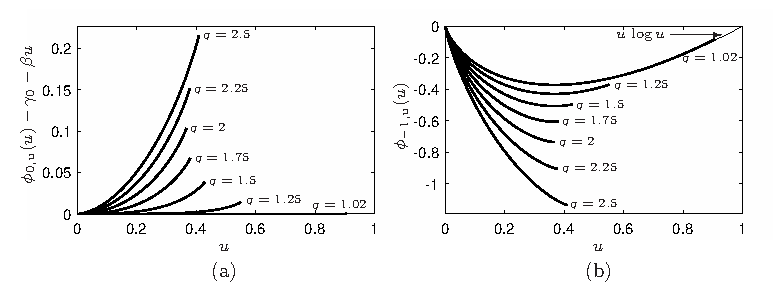
\includegraphics[width=.78\textwidth]{PDF/MaxEnt_GammaLaw}}
\caption{Multiform  entropy   functional  $\phi_\u$   derived  from   the  gamma
  distribution   with  the   partial  moment   constraints  $T_{k,1}(x)   =  x^2
  \un_{\X_k}(x)$, $k\in\{0,-1\}$.  (a): $q = 2$; (b): $q = 5$.}
\label{fig:Entropy-gamma} 
\end{figure}


% ------------------------------- Bibliography ------------------------------- %
% ---------------------------------------------------------------------------- %

%\end{paracol} % To 'close' the left column open by the frontpage...
\reftitle{References}
\externalbibliography{yes}
\bibliography{New_entropies}



% --------------------------------- Biography -------------------------------- %
% ---------------------------------------------------------------------------- %

%% If authors have biography, please use the format below
%\Avoir{
%  \section*{Short Biography of Authors}
%\bio
%{\raisebox{-0.35cm}{\includegraphics[width=3.5cm,height=5.3cm,clip,keepaspectratio]{PhotoSteeve}}}
%{\textbf{Steeve Zozor} Biography of first author}
%%
%\bio
%{\raisebox{-0.35cm}{\includegraphics[width=3.5cm,height=5.3cm,clip,keepaspectratio]{PhotoSteeve}}}
%  {\textbf{Jean-Fran\c{c}ois Bercher} Biography of second author}
%  }

\end{document}
